\documentclass[a4paper,11pt]{article}
\usepackage{fullpage}
\usepackage{graphicx}



\usepackage{amsmath}

\title{\textbf{Advanced Functional Programming \\
    Uppsala University -- Autumn 2012 \\
    Project: Game of Life
  }
}

\author{Anders Hassis \and Jonatan Jansson}

\date{\today}

\begin{document}

\maketitle

\section{Background}

The universe of the Game of Life is a two-dimensional grid of square cells, each of which is in one of two possible states, live or dead. Every cell interacts with its eight neighbours, which are the cells that are horizontally, vertically, or diagonally adjacent. At each step in time, the following transitions occur:

\begin{itemize}
\item Any live cell with fewer than two live neighbours dies, as if by under-population.
\item Any live cell with two or three live neighbours lives on to the next generation.
\item Any live cell with more than three live neighbours dies, as if by overcrowding.
\item Any dead cell with exactly three live neighbours becomes a live cell, as if by reproduction.
\end{itemize}

\noindent We are to implement this in Erlang.

\section{Design}

\subsection{Data representation}
The input to our program is represented as a list of \texttt{\{X,Y\}} tuples containing coordinates. Our internal data is represented as a single list using the indices of the list as a one dimensional representation of the grid. This was chosen over representing the game and input as multidimensional arrays for simplicity.

Note that the worst random access time of a list compared to an array is negligible as random access is only required once during the setup.

\subsection{Synchronization}
To keep our game in sync and avoid race conditions we use a "master" process to notify all cells when a new tic begins. Each cell responds by sending its current state to all its neighbours, then wait for the neighbours to send their state. When all states have been collected, the current cell state is updated and drawn. This avoids synchronization issues by making sure all processes start at roughly the same time. 

\section{User Interface}
We use a web browser for displaying our game state and a library constructed by Sven-Olof Nyström in 2010. The library takes a \texttt{Width} and a \texttt{Height} and generates a frame in that given size and exposes it to the local web browser at the address \texttt{http://localhost:8088/}

We can then use a global variable named \texttt{frame} that we can update a specific cell at a specific coordinate and change its background.

\section{Run cases}
To run and compile game of life, run all of the following:
\begin{itemize}
\item \texttt{c(ehtml).}
\item \texttt{c(frame).} 
\item \texttt{c(gol).}
\end{itemize}

You are now ready to enter your Game of Life simulation. The simulation can be viewed in a web browser at \texttt{http://localhost:8088/}

\subsection{Pulsar}
To run the Pulsar test case, paste the following:

\begin{verbatim}
gol:gol(40,40,[{4,1},{5,1},{6,1},{10,1},{11,1},{12,1},{2,3},{7,3},{9,3},{14,3},
{2,4},{7,4},{9,4},{14,4},{2,5},{7,5},{9,5},{14,5},{4,6},{5,6},{6,6},{10,6},{11,6},
{12,6},{4,8},{5,8},{6,8},{10,8},{11,8},{12,8},{2,9},{7,9},{9,9},{14,9},{2,10},
{7,10},{9,10},{14,10},{2,11},{7,11},{9,11},{14,11},{4,13},{5,13},{6,13},{10,13},
{11,13},{12,13}]).
\end{verbatim}

\noindent That will generate the following simulation:


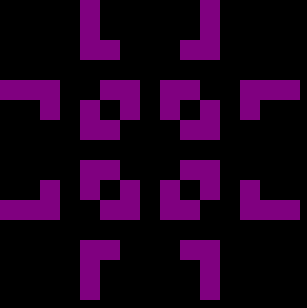
\includegraphics[width=0.3\textwidth]{img/pulsar3.png}

\includegraphics[width=0.3\textwidth]{img/pulsar2.png}

\includegraphics[width=0.3\textwidth]{img/pulsar1.png}


\noindent For more examples, check the bottom of \texttt{gol.erl}


\section{Known bugs}
The update rate for the browser is not in sync with the actual game update. This causes some irregular behaviour in the visualization of the game.



\end{document}
